\documentclass[14pt,aspectratio=1610]{beamer}
\usepackage[utf8]{inputenc}
\usepackage[ngerman]{babel}
\uselanguage{ngerman}
\languagepath{ngerman}
\usetheme{simple}
\usecolortheme{whiteonblack}
\usepackage{array}
\usepackage{url}
\usepackage{graphicx}
\usepackage{csquotes}
\usepackage{amssymb}
\newcommand{\xmark}{\ding{55}}%
\usepackage{pifont}
\newcolumntype{H}{>{\setbox0=\hbox\bgroup}c<{\egroup}@{}} % comment out columns
\author{\texorpdfstring{Konrad Höffner\newline\url{konrad.hoeffner@imise.uni-leipzig.de}}{Konrad Höffner}}
\title{SNIK Ontologie---Lehre und Implementierung}
\subtitle{\url{https://github.com/KonradHoeffner/latex/tree/master/beamer/2016/snik-projekttreffen}}
\begin{document}
\begin{frame}
\titlepage
\end{frame}

\begin{frame}{Vorstellung}
\only<1>
{
\begin{itemize}
\item Konrad Höffner
\item Studium Diplominformatik an Uni Leipzig
\item Doktorand der Informatik beim AKSW, Uni Leipzig/InfAI
\item Thema \enquote{Question Answering auf RDF Data Cubes}
\item bei IMISE und im SNIK Projekt seit Juli
\item kein Vorwissen über Medizin aber viel praktische Erfahrung mit Semantic Web-Technologien
\end{itemize}
}
\only<2>
{
\begin{itemize}
\item Visualisierung, Implementierung, Serialisierung
\item Qualitätssicherung
\item Aufsetzen von Services
\vspace{1em}
\item Raum 227, Tel. (0341)97-16363
\item \href{mailto://konrad.hoeffner@imise.uni-leipzig.de}{konrad.hoeffner@imise.uni-leipzig.de}
\item \url{https://github.com/KonradHoeffner/latex/tree/master/beamer/2016/snik-projekttreffen}
\end{itemize}
}
\end{frame}

\section{Einsatz in der Lehre}

\begin{frame}{}
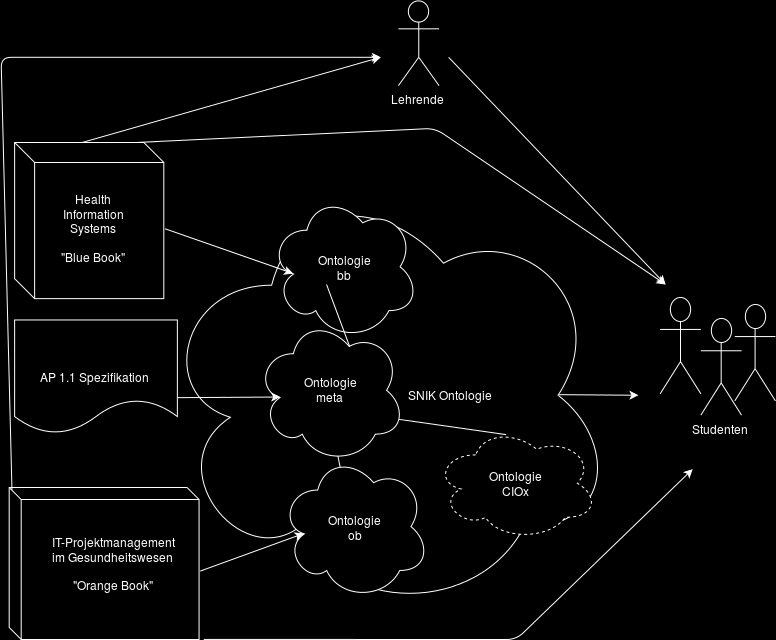
\includegraphics[width=\textwidth,height=0.9\textheight,keepaspectratio]{img/lehre.png}
\end{frame}

\begin{frame}{Ziele}
\begin{itemize}
\item modelliertes Wissen vermitteln, zusätzlich zu Lehrbüchern, Vorlesungen und Übungen
\item Exploration 
\item Erstellen von Übungsaufgaben
\item Semantic Web nur Mittel zum Zweck, so viel Zeit wie möglich für Gesundheitsinformationssysteme 
\end{itemize}
\end{frame}

\begin{frame}{Problem}
\begin{itemize}
\item Studenten sind zwar (Medizin-)Informatiker, haben aber nicht zwangsweise die Semantic Web Vorlesungen von Prof. Fähnrich besucht
\item $\rightarrow$ kein Vorwissen in SPARQL und RDF-Serialisierungsformaten vorauszusetzen
\item Protégé kein intuitiver Gesamtüberblick, getestete Graphplugins skalieren nicht
\end{itemize}
\end{frame}

\begin{frame}{Lösung: Graphvisualisierung}
\begin{block}{Anforderungen}
\begin{itemize}
\item performant bei mehreren tausend Knoten und Kanten 
\item keine Installation nötig 
\item Suchfunktion
\item Filterung
\item Operationen wie kürzeste Wege, \emph{Spiderworm}
\end{itemize}
\end{block}
\begin{block}{Implementierung}
\begin{itemize}
\item Javascript 
\item mehr in Teil 2 (15:45)
\end{itemize}
\end{block}
\end{frame}

\begin{frame}{\url{http://www.snik.eu/(p)graph/}}
\begin{itemize}
\item Öffentliche alte Version ohne CIOx \url{http://www.snik.eu/graph/}
\item Passwortgeschützte neue Version mit CIOx \url{http://www.snik.eu/pgraph/}
\end{itemize}
\end{frame}

\begin{frame}{}
\centering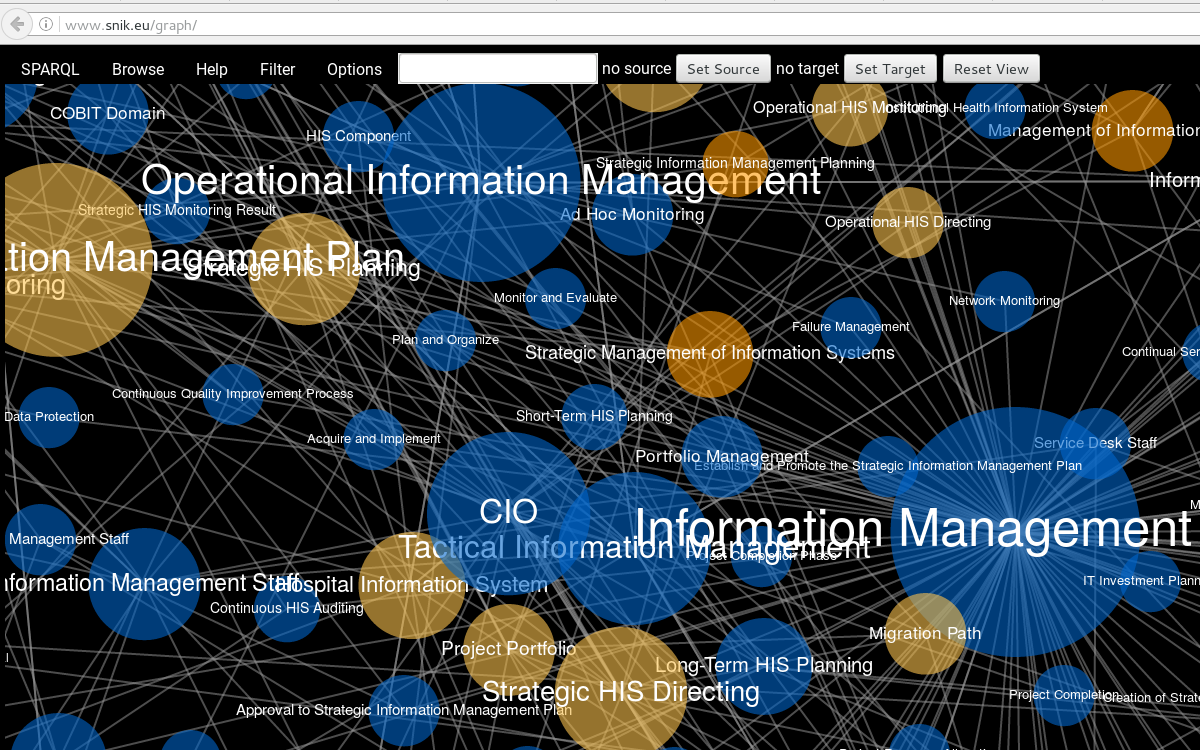
\includegraphics[width=1.05\textwidth,height=1.05\textheight,keepaspectratio]{img/browser.png}
\end{frame}

\begin{frame}{}
\centering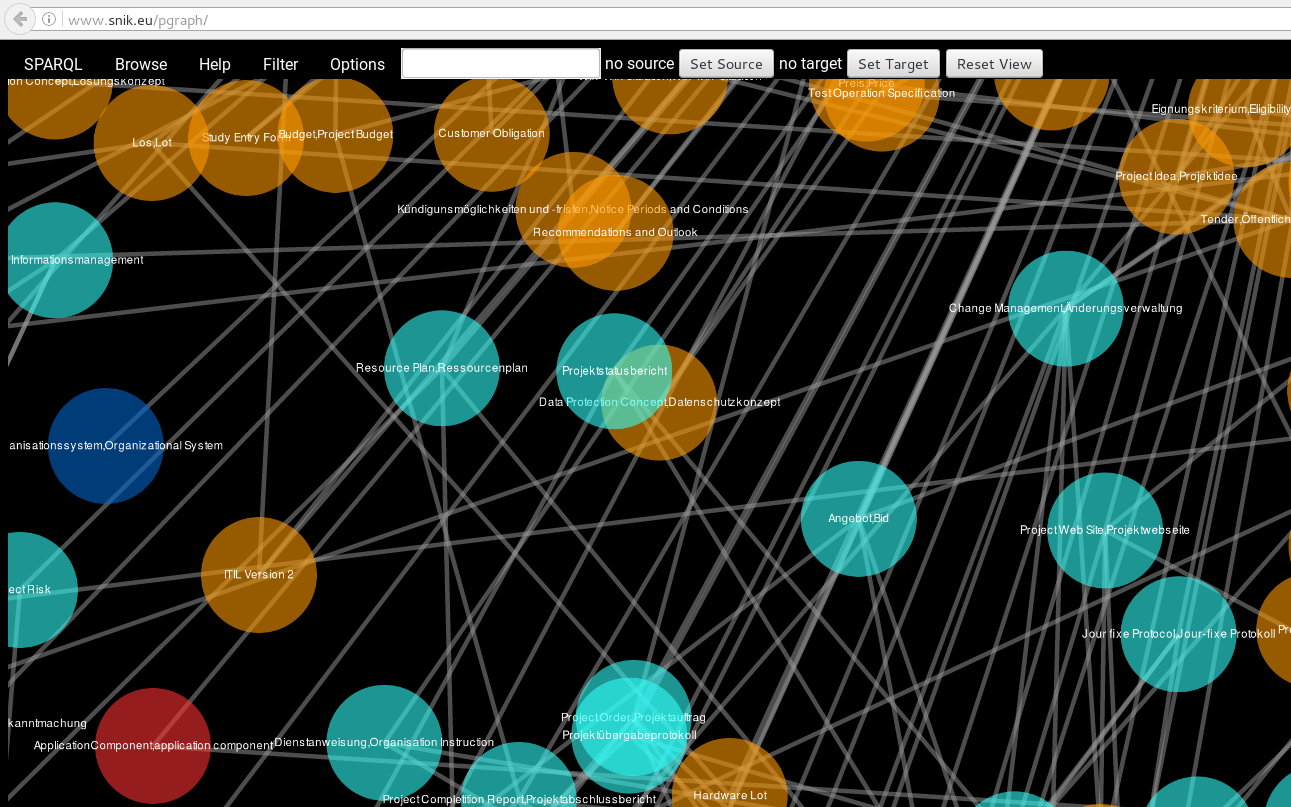
\includegraphics[width=1.05\textwidth,height=1.05\textheight,keepaspectratio]{img/pbrowser.png}
\end{frame}

\begin{frame}{}
\centering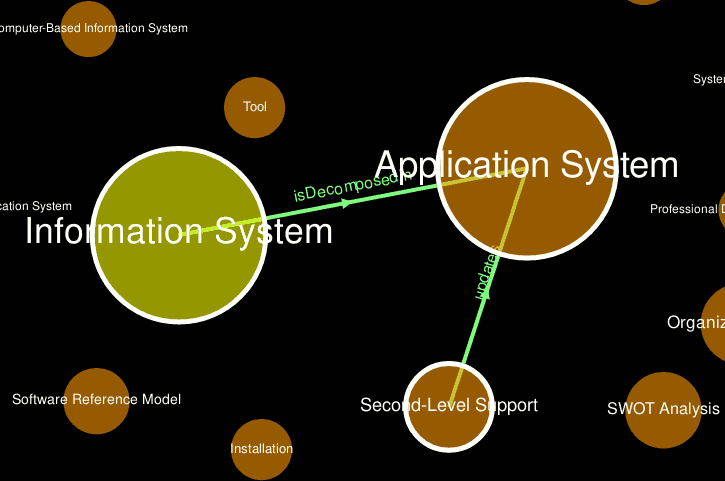
\includegraphics[width=1.05\textwidth,height=1.05\textheight,keepaspectratio]{img/shortestpath.png}
\end{frame}

\begin{frame}{}
\centering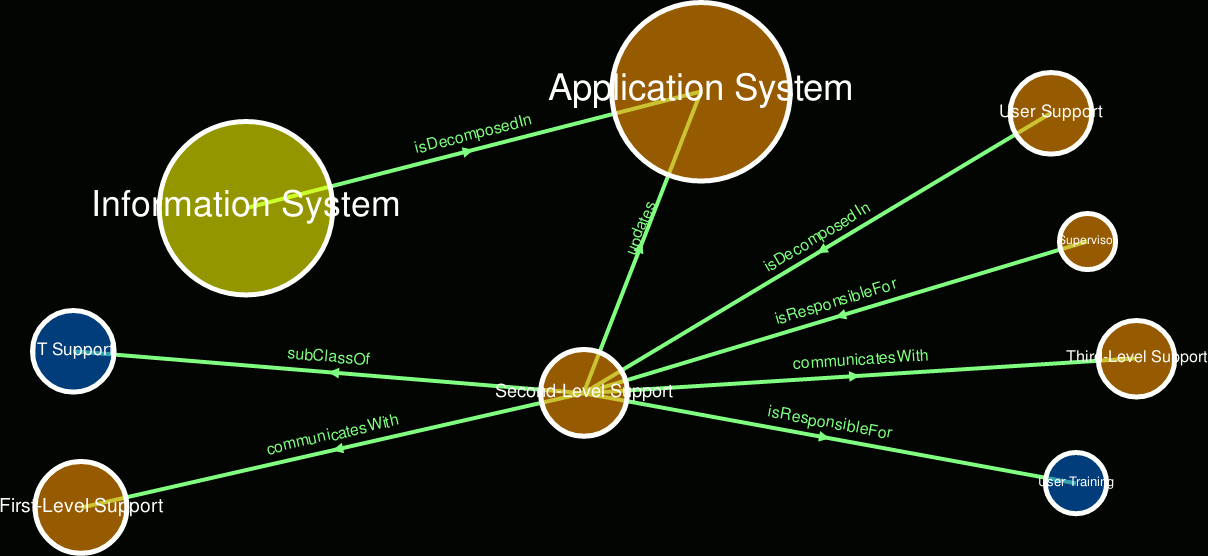
\includegraphics[width=1.05\textwidth,height=1.05\textheight,keepaspectratio]{img/spiderworm.png}
\end{frame}


\section{Implementation}

\begin{frame}{Vokabulare}
\small
\begin{tabular}{lll}
ov		&\url{http://open.vocab.org/terms/}		&Ontologiedefinition\\
%vann		&\url{http://purl.org/vocab/vann/}	&\\%too little usage
skos		&\url{http://www.w3.org/2004/02/skos/core\#}	&Interlinks, Definitionen\\
dc		&\url{http://purl.org/dc/terms}			&Metadaten\\
bibo		&\url{http://purl.org/ontology/bibo/}		&Bibliographie\\
%		&\url{}					&\\
\end{tabular}
\end{frame}

*** TO INSERT ***
https://bitbucket.org/imise/snik-ontology
https://bitbucket.org/imise/snik-ontology/issues
https://bitbucket.org/imise/snik-ontology/downloads/snik.js
select ?x {?x rdfs:subClassOf meta:Function.}
select ?x {?x rdfs:subClassOf* meta:Function.}
Firefox Addon \href{CORS Everywhere}{https://addons.mozilla.org/en-US/firefox/addon/cors-everywhere/}
\begin{frame}{2015--now Other Work}
work
- zweisprachig (englisch und deutsch)
- synonyme -> bessere suchfunktion
- suchfunktion im javascript basiert auf bif:contains, nutzt virtuoso index, ist schnell
- nachteil: muss exakt vorkommen, edit distance = 0
- future work: edit distance > 1, z.B. mit apache lucene/solr index


design decisions
- rdfs:label vs skos:altLabel: ausgeschriebenes ist rdfs:label, abkürzung skos:altLabel (z.B. CIO, chief information officer)
- aussagen über aussagen mit owl axiomen
- triple page
- materialisierung von transitiven properties wie rdfs:subclassOf, hier kann man: nichts materialisieren, alles materialisieren, meta oberklasse materialisieren (Role,Function,...)
-> nichts materialisierung, weil sonst visualisierung unübersichtlich, es gibt sparql 1.1 property paths


probleme:
owl modellierung und rdf-serialisierung/sicht
- protege zeigt gut an aber andere rdf tools haben probleme mit vielen owl statments
beispiel owl restriction -> some ... -> blanknodes, komplizierte visualisierung, ist aber nötig wegen meta-ontologie
bei modellierung wurde mehr wert auf owl gelegt, bei anwendung dann aber eher rdf

aufteilung:
meta ontologie für gemeinsam verwendete begriffe


future work:
- bessere bibliographie (ohne eigenes vokabular mit triple page und so)

\begin{itemize}
\item Supervisor for Software Engineering Student Internship \enquote{Interactive Budget Calculator for the City of Leipzig}
\item Creation of QALD 6 Task 3 Benchmark (QA on RDF Data Cubes)
\item GeoKnow service administration (Website, Wiki, Blog)
\item GeoKnow documentation and Handbook
\item GeoKnow chapter for \enquote{The Semantic Web in Earth and Space Science}
\item Reviews for KESW, SWJ, $\ldots$
\item aksw.org Website Data Officer MOLE
\end{itemize}
\end{frame}

\begin{frame}{2015--now }
\begin{block}{What went well}
\begin{itemize}
\item QA Survey (thanks for all the help!) 
\item Coauthorships 
\item Other Work 
\end{itemize}
\end{block}
\begin{block}{What didn't}
\begin{itemize}
\item publication of CubeQA long version
\end{itemize}
\end{block}
\end{frame}

\begin{frame}{Thanks \& Outlook}
\begin{itemize}
\item thanks to Jens, other coauthors and other people who give help and advice
\end{itemize}
\begin{block}{Outlook}
\begin{enumerate}
\item coauthor papers with Edgard, Diego E. and André(?) until reviews are in, then rebuttal
\item write 4th core paper to have enough thesis material
\item write thesis, defend
\item ?
\end{enumerate}
\end{block}
\end{frame}

\begin{frame}{Unrelated Proposal: Virtual Paper Review}
Workflow at the moment: finish papers at last moment and only review among coauthors.
\only<1>
{
\begin{block}{Problem}
\begin{itemize}
\item In case of emergencies no paper 
\item Authors and coauthors know what the paper is about and thus cannot judge understandability.
\end{itemize}
\end{block}
}
\only<2>
{
\begin{block}{Solution}
\begin{itemize}
\item Virtual deadline one week before real one
\item Coworkers who are not coauthors review it
\item Submitted paper is then already revised 
\end{itemize}
\end{block}
}
\end{frame}


\end{document}
